\documentclass{beamer}
\usetheme[pageofpages=of,% String used between the current page and the
                         % total page count.
          bullet=circle,% Use circles instead of squares for bullets.
          titleline=true,% Show a line below the frame title.
          alternativetitlepage=true,% Use the fancy title page.
       %   titlepagelogo=logo-polito,% Logo for the first page.
       %   watermark=watermark-polito,% Watermark used in every page.
       %   watermarkheight=100px,% Height of the watermark.
       %   watermarkheightmult=4,% The watermark image is 4 times bigger
                                % than watermarkheight.
          ]{Torino}

\setbeamertemplate{footline}{
  \begin{beamercolorbox}[wd=\paperwidth,ht=1ex,dp=1ex]{footline}
    \vspace{5pt} \hspace{1em} \insertframenumber/\inserttotalframenumber
  \end{beamercolorbox}
}

\author{Brendon J. Brewer}
\title{STATS 331 -- Introduction to Bayesian Statistics}
\institute{The University of Auckland}
\date{}


\linespread{1.3}
\usepackage{minted}
\usepackage[utf8]{inputenc}
\usepackage{dsfont}


\begin{document}

\frame{\titlepage}

\begin{frame}
\frametitle{Welcome}
This lecture will just give an overview of the course.

\end{frame}


% New slide
\begin{frame}
\frametitle{Famous Bayesian Figures}

\begin{figure}[!h]
\centering
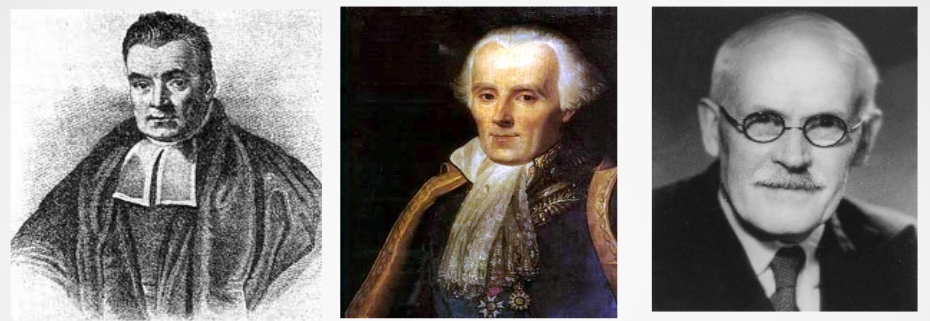
\includegraphics[width=0.8\textwidth]{images/people.png}
\caption{Thomas Bayes, Pierre-Simon Laplace, Harold Jeffreys
\label{fig:people}}
\end{figure}

\end{frame}


% New slide
\begin{frame}
\frametitle{Practicalities}
There are only two lectures per week, along with two lab sessions.
You should generally only come to one lab session, unless you want extra help. \\[1em]
\pause

All the course material will be available on Canvas.

\end{frame}


% New slide
\begin{frame}
\frametitle{Labs}

\begin{alertblock}{Lab Start Date}
There are no labs in Week 1. Labs will begin in Week 2.
\end{alertblock}\pause

\begin{alertblock}{Lab Attendance}
Lab attendance is not mandatory, but it will be much easier to
fully understand the material if you attend and attempt the questions.
\end{alertblock}

\end{frame}


% New slide
\begin{frame}
\frametitle{Grades and Assessment}
The grades available in this course are broken down as follows:\pause

\begin{itemize}
\item 24\% Assignments (Four assignments, each worth 6\%)\pause
\item 6\% Canvas quizzes (Two quizzes, each worth 3\%)\pause
\item 20\% Midterm Test (held in Week 7)\pause
\item 50\% Final Exam (two hours)\pause
\end{itemize}

\begin{alertblock}{Exam Minimum}
You must achieve 45\% on the final exam, as well as 50\% overall, to pass.
There is no plussage.
\end{alertblock}
\end{frame}


% New slide
\begin{frame}
\frametitle{The Four Assignments}
\begin{itemize}
\item The assignments will be uploaded to Canvas at least two weeks before they
are due.
\item The assignments are intended to be of medium difficulty and length.
\item Assignment submission will be via PDF upload on Canvas.
\end{itemize}

\end{frame}




% New slide
\begin{frame}
\frametitle{Class Representative}
We will need a class representative. Please see me at the end of this lecture
if you would like to volunteer. You will need to be available at the time of the
meetings.


\end{frame}


% New slide
\begin{frame}
\frametitle{Office Hours}
I will run one office hour each week, where you can ask me anything about the
course, including assignment help. The exact hour will be posted on Canvas. \pause

\begin{alertblock}{Office Location}
My office is room 331 (!) in Building 303 (the Science building).
\end{alertblock}
\end{frame}


% New slide
\begin{frame}
\frametitle{Lecture Notes and Books}
There are some PDF lecture notes (written a long time ago now, but with a
couple of recent updates) available on Canvas. These notes cover much of
the same material as lectures, but there are some topics that do not appear in
the notes.\\[1em] \pause

I will also suggest a couple of books which might be helpful.
\end{frame}


\begin{frame}
\frametitle{Books}
The book {\em Doing Bayesian Data Analysis: A Tutorial with R, JAGS, and Stan}
by John Krushcke covers roughly similar ground to STATS 331.
Plus it has dogs for some reason.

\begin{figure}[!h]
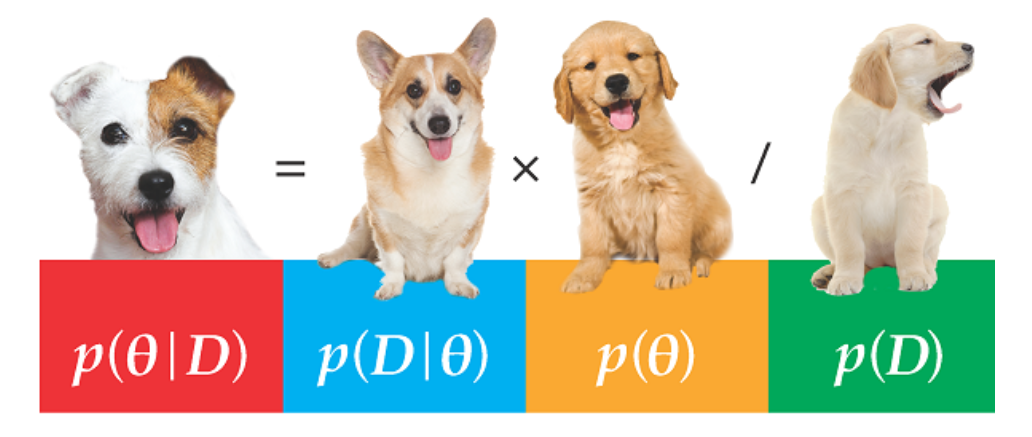
\includegraphics[width=0.7\textwidth]{images/dogs.png}
\caption{Dogs.\label{fig:dogs}}
\end{figure}



\end{frame}

\end{document}

